\documentclass[9pt]{extarticle}
% (1) Encoding, Fonts, and Layout
\usepackage[T1]{fontenc}
\usepackage{lmodern}
\usepackage[margin=1in]{geometry}


% (2) Common Packages
\usepackage{amsmath, amssymb, amsthm}
\usepackage{xcolor}
\usepackage{caption}
\usepackage{tikz}
\usepackage{pgfplots}
\pgfplotsset{compat=newest}
\usepackage{etoolbox}
\usepackage{tikz-3dplot}
\tdplotsetmaincoords{75}{120}
\usepackage[inline]{enumitem}
\usepackage{bookmark}
\usepackage{mathtools}
\usepackage{subcaption} % For subfigures
\usepackage[normalem]{ulem} % For better underline commands

% Micro-typography
\usepackage{microtype}

% Patching pgfplots warning
\makeatletter
\patchcmd{\pgfplots@applistXXpushback@smallbuf}{\pgfplots@error}{\pgfplots@warning}{}{}
\makeatother

% (3) tcolorbox and Theorem Libraries
\usepackage{tcolorbox}
\tcbuselibrary{theorems}

% (4) Define Colors
\definecolor{custom_green}{HTML}{a3be8c}
\definecolor{custom_red}{HTML}{dc322f}
\definecolor{custom_blue}{HTML}{268bd2}
\definecolor{custom_purple}{HTML}{b48ead}

\definecolor{base}{HTML}{eceff4}
\definecolor{gray1}{HTML}{e5e9f0}
\definecolor{gray2}{HTML}{d8dee9}
\definecolor{gray3}{HTML}{2e3440}
\pagecolor{base}

% (5) Custom tcolorbox Environments
\newtcolorbox{definitionbox}[1][]{
    title=\textbf{Definition} {#1},
    fonttitle=\bfseries\boldmath,
    arc=0mm,
    bottomtitle=0.5mm,
    boxrule=0mm,
    colbacktitle=gray2,
    colback=gray1,
    coltitle=gray3,
    coltext=gray3,
    left=2.5mm,
    leftrule=1mm,
    rightrule=1mm,
    right=3.5mm,
    toptitle=0.75mm,
    colframe=custom_red,
}

\newtcolorbox{proofbox}{
    title=\textbf{Proof},
    fonttitle=\bfseries\boldmath,
    arc=0mm,
    bottomtitle=0.5mm,
    boxrule=0mm,
    colbacktitle=gray2,
    colback=gray1,
    coltitle=gray3,
    left=2.5mm,
    leftrule=1mm,
    rightrule=1mm,
    right=3.5mm,
    toptitle=0.75mm,
    colframe=custom_blue,
    coltext=gray3,
}

\newtcolorbox{theorembox}[1][]{
    title=\textbf{Theorem} {#1},
    fonttitle=\bfseries\boldmath,
    arc=0mm,
    bottomtitle=0.5mm,
    boxrule=0mm,
    colbacktitle=gray2,
    colback=gray1,
    coltitle=gray3,
    left=2.5mm,
    leftrule=1mm,
    rightrule=1mm,
    right=3.5mm,
    toptitle=0.75mm,
    colframe=custom_green,
    coltext=gray3
}

\newtcolorbox{notebox}{
    title=\textbf{Note},
    fonttitle=\bfseries\boldmath,
    arc=0mm,
    bottomtitle=0.5mm,
    boxrule=0mm,
    colbacktitle=gray2,
    coltitle=gray3,
    left=2.5mm,
    leftrule=1mm,
    rightrule=1mm,
    right=3.5mm,
    toptitle=0.75mm,
    colframe=custom_blue,
    coltext=gray3
}

\newtcolorbox{examplebox}[1][]{
    title=\textbf{Example} {#1},
    fonttitle=\bfseries\boldmath,
    arc=0mm,
    bottomtitle=0.5mm,
    boxrule=0mm,
    colbacktitle=gray2,
    colback=gray1,
    coltitle=gray3,
    left=2.5mm,
    leftrule=1mm,
    rightrule=1mm,
    right=3.5mm,
    toptitle=0.75mm,
    colframe=gray3,
    fontupper=\footnotesize,
    coltext=gray3
}

% (6) Theorem Environments
\theoremstyle{definition}
\newtheorem{definition}{Definition}[section]
\newtheorem{example}[definition]{Example}

\theoremstyle{plain}
\newtheorem{theorem}[definition]{Theorem}

% (7) Hyperlinks
\usepackage{hyperref}
\hypersetup{
    colorlinks=true,    % Use colored text for links
    linkcolor=custom_red,      % Set link text color to red
    pdfborder={0 0 0}   % Remove the default box around links
}

% macros.tex
\newcommand{\intinf}{\int_0^{\infty}} % Integral from 0 to infinity
\newcommand{\diff}[2]{\frac{d#1}{d#2}} % Derivative


\usepackage[svgnames]{xcolor}
\usepackage{listings}


\title{
Robert Davidson \\
\textbf{ST1112: Statistics}
}
\author{
70\% Exam\\
30\% Continuous Assessment (3 parts)
}
\date{}       % Optional: Add date if desired
%--------------------------------------------------------
% Document
%--------------------------------------------------------
\begin{document}
\maketitle
\pagebreak

\tableofcontents
\pagebreak

\section{Inferential Statistics - Interval Estimation}
The ultimate goal in statistical inference is to estimate population parameters (like the mean $\mu$) based on sample statistics (like the sample mean $\bar{X}$).
\subsection{Probability vs Statistics}
\begin{itemize}
    \item \textbf{Probability} deals with known underlying processes: one starts with a model (like proportion of red vs. green jelly beans in a jar) and computes probability of specific outcomes
    \item \textbf{Statistics} works in reverse: one observes outcomes (sample data) and attempts to infer the underlying process or population parameters (e.g. proportion of red jellybeans)
\end{itemize}
\subsection{Definitions and Concepts}

\begin{definitionbox}{Population}{}
    A \textbf{population} is the complete set of items (or individuals) of interest.
\end{definitionbox}

\begin{definitionbox}{Sample}{}
    A \textbf{sample} is a subset of that population, intended to represent the population\\

    For example the sample mean $\bar{X}$ is an estimate of the population mean $\mu$.
\end{definitionbox}

\begin{definitionbox}{Population Mean ($\mu$)}{}
    $\mu$ represents the central tendency of a population distribution.
    $$\mu = \frac{1}{N} \sum_{i=1}^{N} x_i$$
    where $N$ is the population size and $x_i$ are the individual values in the population.\\

    $\mu$ is sometimes called the expected value or average.
\end{definitionbox}

\begin{definitionbox}{Population standard deviation ($\sigma$)}{}
    $\sigma$ measures the dispersion or spread of values around the mean in a population.
    $$\sigma = \sqrt{\frac{1}{N} \sum_{i=1}^{N} (x_i - \mu)^2}$$
    where $N$ is the population size and $x_i$ are the individual values in the population.\\
\end{definitionbox}

\begin{conceptbox}{Sampling Variation}{}
    When we take multiple samples from the same population, each sample's mean $\bar{X}$ will be different. This is variability is called \textbf{sampling variation}. \\

    Larger sample sizes tend to reduce this variation, that is as $n$ gros, the sample mean $\bar{X}$ becomes a better estimate of the population mean $\mu$.
\end{conceptbox}
\begin{conceptbox}{Sampling Distributions}{}
    The sample mean itself is a \textbf{random variable} because different samples yield different mean values.\\

    The distribution of all possible sample means (of a given sample size $n$) is called the \textbf{sampling distribution} of the sample mean ($\bar{X}$).
\end{conceptbox}

\begin{definitionbox}{Expected Value of the Sample Mean}{}
    $$E(\bar{X}) = \mu$$
    This means if you averaged all possible sample means, you would get the population mean $\mu$.
\end{definitionbox}
\begin{definitionbox}{Standard Error of the Mean}{}
    $$SE = SD(\bar{X}) = \frac{\sigma}{\sqrt{n}}$$
    where $\sigma$ is the population standard deviation and $n$ is the sample size.\\

    This value is called the \textbf{standard error} of the mean and measures how much the sample mean $\bar{X}$ fluctuates around the population mean $\mu$.
\end{definitionbox}

\begin{definitionbox}{Central Limit Theorem}{}
    $$\bar{X} \sim N\left(\mu, \frac{\sigma^m}{n}\right)$$
    where $\bar{X}$ is the sample mean, $\mu$ is the population mean, and $\sigma$ is the population standard deviation.\\

    The \textbf{Central Limit Theorem} states that the sampling distribution of the sample mean $\bar{X}$ (the distribution of all sample means)  approaches a normal distribution as the sample size $n$ increases, \textbf{regardless of the shape of the population distribution.}\\

    This means that for large enough sample sizes, we can use the normal distribution to make inferences about the population mean $\mu$. \\

    \textbf{Practically}, many apply the rule of thumb $n \geq 30$ to treat $\bar{X}$ as normally distributed.
\end{definitionbox}


\begin{definitionbox}{Unbiased Estimators}{}
    We say a statistic $T$ is an \textbf{unbiased estimator} of a population parameter $\theta$,  if $E(T) = \theta$.\\

    For example, the sample mean $\bar{X}$ is an unbiased estimator of the population mean $\mu$ because $E(\bar{X}) = \mu$.\\

    The sample standard deviation $s$ (using Bessel's correction, dividing by multiplying by $\frac{1}{n-1}$ rather than $\frac{1}{N}$) is an unbiased estimator of the population standard deviation $\sigma$.
\end{definitionbox}

\subsection{Example}
\begin{examplebox}{Weekly rent}{}
    If a population mean rent is $\mu = 225$, with $\sigma = 25$ for a population sample size $n = 30$, the sample distribution of the sample mean is approximately:
    $$\bar{X} \sim N\left(225, \frac{25^2}{30}\right)$$
    This lets us compute probabilities for specific sample mean ranges using the normal distribution (e.g. $P(\bar{X} < 220)$).
\end{examplebox}
\subsection{Recap}
A \textbf{sample statistic} (e.g. the sample mean $\bar{X}$) varies from one sample to another. Understanding this variation (and quantifying it via the standard error) is crucial for knowing how precise (or imprecise) an estimate really is. \\[2ex]
If we have a large sample size $n$ from a population with mean $\mu$ and standard deviation $\sigma$, then our sample distribution of the sample mean $\bar{X}$ is approximately normal:
$$\bar{X} \sim N\left(\mu, \frac{\sigma^2}{n}\right)$$
In practice, for $n \geq 30$, $\bar{X}$ can be treated as normally distributed even if the original population is not strictly normal.
\subsection{Confidence Intervals}
\begin{conceptbox}{Why confidence intervals?}{}
    Why do we need confidence intervals, instead of a single point estimate, like the sample mean $\bar{X}$? \\

    A confidence interval provides a range of plausible values for the population parameter (e.g. $\mu$) based on the sample data. \\

    \textbf{Analogy:}  Using a single point estimate is like trying to catch a fish wih a spear; your aim may not be perfect. Using a confidence interval is like using a net; we have a better chance of "catching" (capturing) the true population parameter.
\end{conceptbox}
\begin{definitionbox}{Confidence Interval}{}
    $$\bar{X} \pm (\text{critical value}) \times SE(\bar{X})$$
    where $SE(\bar{X}) = \frac{\sigma}{\sqrt{n}}$ is the standard error of the sample mean, $\pm$ is the margin of error. \\
    The general formula for a desired confidence level 100(1- $\alpha$)\% is:
    $$\bar{X} \pm z_{\alpha/2} \times \frac{\sigma}{\sqrt{n}}$$
    where $z_{\alpha/2}$ is the critical value from the standard normal distribution.
\end{definitionbox}
\noindent\textbf{Interpretation}: \\
If we repeat the sampling process many times and construct confidence intervals from each sample, then approximately $100 \times (1 - \alpha)\%$ of those intervals will contain the true population parameter $\mu$.\\
In other words, you do not say \emph{"there is a 95\% chance that $\mu$ lies in my interval"}. Rather we say, \textbf{"on repeated sampling 95\% of such intervals will contain the true population mean $\mu$."}


\begin{definitionbox}{Critical Values}{}
    The \textbf{critical value} is a z-score that corresponds to the desired confidence level. \\[2ex]
    For example, for a 95\% confidence level, the critical value is $Z_{\alpha/2} = 1.96$ (where $\alpha = 0.05$).
    This means that 95\% of the area under the normal curve lies within $1.96$ standard deviations of the mean. \\[2ex]
    \begin{center}
        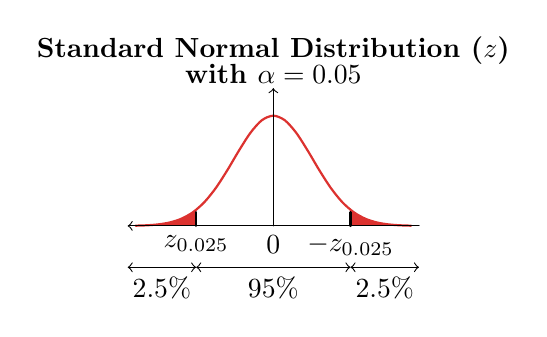
\begin{tikzpicture}[
                domain=-1:1,
                xscale=-0.5,
                yscale=3.5,
                smooth,
                line cap=round,
                line join=round,
            ]
            % Define critical z values
            \def\zcrit{1.96}

            % Fill left tail area (2.5%)
            \fill[custom_red] (-3.5,0) -- plot[domain=-3.5:-\zcrit] (\x, {0.4*exp(-(\x)^2/2)}) -- (-\zcrit,0) -- cycle;

            % Fill right tail area (2.5%)
            \fill[custom_red] (3.5,0) -- plot[domain=3.5:\zcrit] (\x, {0.4*exp(-(\x)^2/2)}) -- (\zcrit,0) -- cycle;

            % Draw the normal distribution curve
            \draw[thick, custom_red] plot[domain=-3.5:3.5] (\x, {0.4*exp(-(\x)^2/2)});

            % Mark the critical values
            \draw[thick] (-\zcrit,0) -- (-\zcrit,0.05);
            \node[below] at (-\zcrit,0) {$-z_{0.025}$};
            \draw[thick] (\zcrit,0) -- (\zcrit,0.05);
            \node[below] at (\zcrit,0) {$z_{0.025}$};

            \draw[<->] (-\zcrit, -0.15) -- (\zcrit, -0.15) node[midway, below] {$95\%$};
            \draw[<->] (-\zcrit, -0.15) -- (-3.7, -0.15) node[midway, below] {$2.5\%$};
            \draw[<->] (\zcrit, -0.15) -- (3.7, -0.15) node[midway, below] {$2.5\%$};


            % Draw horizontal axis
            \draw[->] (-3.7,0) -- (3.7,0) node[right] {};
            % Draw vertical axis
            \draw[->] (0,0) -- (0,0.5) node[above] {};
            % Mark the center
            \node[below] at (0,0) {$0$};
            % Title
            \node[above] at (0,0.55) {\textbf{Standard Normal Distribution ($z$)}};
            \node at (0,0.55) {\textbf{with $\alpha = 0.05$}};
        \end{tikzpicture}
    \end{center}
\end{definitionbox}

\begin{examplebox}{Find crtitical value for the 95\% CI}{}
    For a confidence interval of 95\%, we want to find the z-score that leaves 2.5\% in each tail of the normal distribution.\\
    We want to find the $z$-value where the cumulative area )from the left up to that $z-score$) is $1 - 0.025 = 0.975$.\\
    We look in the $z$-tables for the value closest to $0.975$ and read the row and column headers to find the $z$-value.\\
    The $z$-value is $1.96$.\\
\end{examplebox}

\begin{examplebox}{Find the 95\% confidence interval for the population mean $\mu$ given}{}
    A dataset of 103 students, of whom 71 pay rent, was used to estimate the average weekly rent $\mu$.
    \begin{itemize}
        \item \textbf{Point estimate}: the sample mean $\bar{X} \approx 546.239$.
        \item \textbf{Sample standard deviation}: $s \approx 187.862$.
        \item \textbf{Sample size}: $n = 71$.
    \end{itemize}
    Confidence Interval is given by:
    $$\bar{X} \pm z_{\alpha/2} \times \frac{s}{\sqrt{n}}\Rightarrow 546.239 \pm 1.96 \times \frac{187.862}{\sqrt{71}}$$
    where $z_{\alpha/2} = 1.96$ for a 95\% confidence level.The resulting confidence interval is:
    $$(502.541, 589.938)$$
    \textbf{Interpretation}: We are 95\% confident that the true mean weekly rent for all NUI Galway students (population) is roughly 503 to 590 euros.
\end{examplebox}
\subsection{Higher Confidence Levels means Wider Intervals}
\begin{itemize}
    \item To achieve a \textbf{higher confidence level}, we need to increase the critical value $z_{\alpha/2}$, which in turn increases the margin of error.
    \item This results in a wider confidence interval, which means we are more certain that the true population parameter lies within that interval.
    \item Conversely a \textbf{lower confidence level} results in a smaller critical value, leading to a narrower confidence interval.
\end{itemize}
\pagebreak
\subsection{t-Distribution}
\begin{conceptbox}{Why the $t-$distribution}{}
    When the sample size is small ($n < 30$) and the population standard deviation $\sigma$ is unknown, simply substituting the sample standard deviation $s$ no longer suffices because the standard error is itself estimated with more uncertainty.\\[2ex]
    The $\textbf{t-distributution has thicker}$ tails than the normal distributution. This extra "fatness" in the tails accounts for the additional uncertainty in using $s$ instead of $\sigma$.
    \begin{center}
        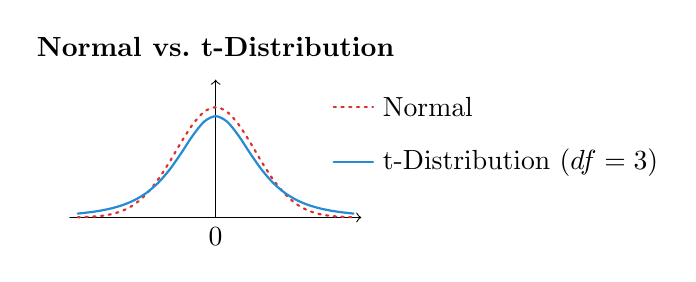
\begin{tikzpicture}[
            domain=-3.5:3.5,
            xscale=0.5,
            yscale=3.5,
            smooth,
            line cap=round,
            line join=round
        ]
            % Draw axes
            \draw[->] (-3.7,0) -- (3.7,0) node[right] {$$};
            \draw[->] (0,0) -- (0,0.5) node[above] {$$};
            \node[below] at (0,0) {$0$};
        
            % Plot the Normal Distribution (dotted red)
            \draw[dotted, thick, custom_red] plot (\x, {0.4*exp(-(\x)^2/2)});
        
            % Plot the t-Distribution (solid blue) for df = 5.
            % The t-density: f(t) = (8/(3*pi*sqrt(5)))*(1+t^2/5)^(-3)
            \draw[thick, custom_blue] plot (\x, {(2/(3.14159*sqrt(3)))*((1+(\x)^2/3)^(-2))});
        
            % Title and legend
            \node[above] at (0,0.55) {\textbf{Normal vs.\ t-Distribution}};
        
            % Legend (placed at the top-right)
            \begin{scope}[shift={(3,0.4)}]
                \draw[dotted, thick, custom_red] (0,0) -- (1,0);
                \node[right] at (1,0) {Normal};
                \draw[thick, custom_blue] (0,-0.2) -- (1,-0.2);
                \node[right] at (1,-0.2) {t-Distribution ($df=3$)};
            \end{scope}
        \end{tikzpicture}        
    \end{center}
\end{conceptbox}
\vfill
\begin{conceptbox}{Degrees of Freedom (df)}{}
    A t-distribution is characterized by its degrees of freedom, where 
    $$df = n - 1 \quad \text{for a sample mean}$$
    As the sample size $n$ increases, the t-distribution approaches the standard normal distribution.\\
    For example, for $n = 30$, $df = 29$ and the t-distribution is very close to the normal distribution.\\
\end{conceptbox}
\vfill
\begin{definitionbox}{Confidece Intervals (t-based)}{}
    $$\bar{X} \pm t_{\alpha/2, df} \times \frac{s}{\sqrt{n}}$$
    where $t_{\alpha/2, df}$ is the critical value from the t-distribution with $df = n - 1$ degrees of freedom - or from a function like \texttt{qt()} in R.\\

    \textbf{Assumption}: The population itself should be approximately normally distributed when using t-based methods for small sample sizes.
\end{definitionbox}
\vfill
\begin{examplebox}{Finding t-critical values}{}
    Find the critical value for a 95\% confidence interval with $n = 12$ (so $df = 11$).\\
    We look for the row associated with $df = 11$ and the column associated with $\alpha/2 = 0.025$.\\
    The critical value is:
    $$t_{0.025, 11} \approx 2.201$$
\end{examplebox}
\pagebreak
\subsection{CI with large $\boldsymbol{n}$, and $\boldsymbol{\sigma}$ unknown}
The $z$-based critical interval is given as:
$$\bar{X} \pm z_{\alpha/2} \times \frac{\sigma}{\sqrt{n}}$$
where $z_{\alpha/2}$ is the critical value from the standard normal distribution.
However, if the population standard deviation $\sigma$ is unknown, we can use the sample standard deviation $s$ as an estimate.\\
This gives us the following confidence interval:
$$\bar{X} \pm z_{\alpha/2} \times \frac{s}{\sqrt{n}}$$
\textbf{Interpretation}: around 95\% of all possible 95\% confidence intervals will contain the true population mean $\mu$. We can visualize that if we drew many repeated samples, sample means will form an overlapping $\mu$ and a small fraction will not.

\subsection{CI with small $\boldsymbol{n}$, and $\boldsymbol{\sigma}$ unknown}
If the sample size is small ($n < 30$) and the population standard deviation $\sigma$ is unknown, we use the t-distribution to construct the confidence interval. This gives us the following confidence interval:
$$\bar{X} \pm t_{\alpha/2, df} \times \frac{s}{\sqrt{n}}$$
where $t_{\alpha/2, df}$ is the critical value from the t-distribution with $df = n - 1$ degrees of freedom.\\
\textbf{Interpretation}: around 95\% of all possible 95\% confidence intervals will contain the true population mean $\mu$. We can visualize that if we drew many repeated samples, sample means will form an overlapping $\mu$ and a small fraction will not.

\begin{examplebox}{Turin Shroud}{}
    A historical cloth's age was tested by carbon dating on 12 pieces ($n = 12$). The sample mean was $x \approx 1261 \ AD$ and the sample standard deviation was $s \approx 61.2 \ AD$. Find the 95\% confidence interval for the population mean age of the cloth. \\[2ex]
    The standard error is given by:
    $$SE = \frac{s}{\sqrt{n}} = \frac{61.2}{\sqrt{12}} \approx 17.67$$
    For a 95\% confidence interval with $n-1 = 11$ degrees of freedom, the critical value is $t_{0.025, 11} \approx 2.201$.\\
    The confidence interval is given by:
    $$\bar{X} \pm t_{\alpha/2, df} \times SE = 1261 \pm 2.201 \times 17.67$$
    The resulting confidence interval is:
    $$(1222, 1300)$$
    \textbf{Interpretation}: The cloth’s true average carbon-dated age is plausibly within about 1222–1300 AD. This range casts doubt on claims that the cloth dates from centuries earlier.
\end{examplebox}
\begin{examplebox}{Unathorized Computer Acess}{}
    Find 95\% CI given:
    \begin{itemize}
        \item \textbf{Data}: 18 times between keystrokes 
        \item \textbf{Sample mean}: $\bar{X} = 0.29$ seconds
        \item Sample standard deviation: $s = 0.0074$ seconds
    \end{itemize}
    $$n  = 18 \Rightarrow df = 17$$
    For a 95\% confidence interval with $n-1 = 18$ degrees of freedom, the critical value is $t_{0.025, 17} \approx 1.740$.\\
    The resulting confidence interval is:
    $$(0.2532, 0.3268)$$
    \textbf{Interpretation}: We are 95\% confident that the true mean time between keystrokes is between 0.2532 and 0.3268 seconds.
\end{examplebox}


\subsection{When normality is questionable}
Recall that for small $n$, the t-distribution-based confidence interval requires data to be approximately normally distributed in the population. But many real datasets violate this assumption. - e.g. skewed data, heavily tailed data etc. \\[2ex]
\noindent Two broad remedies exist:
\begin{itemize}
    \item \textbf{Data transformation}: Apply a mathematical transformation to make the data more symmetric or bell shape (e.g.log-transformation). Then use t-based or z-based methods on the transformed scale.
    \item \textbf{Non-parametric methods}: Rely less on strict distributional assumptions. The bootstrap is a common and versatile non-parametric method approach to estimating confidence intervals and sampling variability.
\end{itemize}

\subsection{Data Transformations}
\textbf{Purpose}:
\begin{itemize}
    \item If the data has a strongly skewed or otherwise non-normal distribution, applying a suitable transformation (e.g. $\log(x)$, $\sqrt{x}$) can help to make the data more symmetric and bell-shaped.
    \item After the transformation, we can apply t-based or z-based methods can be applied more safely.
\end{itemize}
\textbf{Cautions}:
\begin{itemize}
    \item Finding the write transformation can be tricky; sometimes no simple transformation works well.
    \item Interpretation of results becomes more complex; if you compute a CI for the transformed mean, you must convert (e.g. exponentiate) the results back to the original scale.
    \item Despite these challenges, transformation often prove very useful in practice.
\end{itemize} 

\subsection{The Bootstrap}
\textbf{Motivation}:
\begin{itemize}
    \item Bootstrap methods do not require normality assumptions or a large $n$. They rely on the principle that the observed sample can server a reasonable proxy for the populations shape. 
    \item By resampling with replacement from the original sample (many times), one creates a "bootstrap distribution" that mimics the statistic (e.g. mean, median) of interest.
    \item This bootstrap distribution is then used to estimate hpw the statistic varies, allowing for confidence interval construction and hypothesis testing without explicit formulas.
\end{itemize}
\textbf{Basic Steps (Bootstrap Scheme)}
\begin{enumerate}
    \item \textbf{Resample with replacement}: Take a bootstrap sample of the same size $n$ as the original dataset, but drawn from the dataset with replacement.
    \item \textbf{Calculate Bootstrap statistic}: Compute the same summary measure of interest (e.g. mean, median) on the bootstrap sample.
    \item \textbf{Repeat}: Repeat steps (1) and (2) many times (e.g. 1000 times) to create a distribution of the bootstrap statistic.
    \item \textbf{Construct CI}: The bootstrap distribution of the resampled statistics can be used to determine the middle 95\% (or chosen confidence level) as the CI bounds.
\end{enumerate}


\textbf{Advantages}:
\begin{itemize}
    \item Works for all kinds of statistics (mean, median, proportion, regression coefficients, etc.) even when no closed-form CI exists.
    \item Far fewer assumptions about the underlying population distribution.
\end{itemize}
\textbf{Disadvantages}:
\begin{itemize}
    \item Computationally intensive; requires many resamples (e.g. 1000) to get a good approximation.
    \item Requires the sample itself to be a good representation of the population; if the sample is biased, the bootstrap may not work well.
\end{itemize}
\section{Inferential Statistics - Hypothesis Testing}
\subsection*{Recap: Confidence Intervals for a Population Mean}
\vfill
\begin{itemize}
    \item A \textbf{Confidence interval (CI)} provides a range of plausible values for a population parameter
    \item For a large sample ($n \geq 30$) or a known $\sigma$, we often use a z-based interval:
    $$\bar{X} \pm z_{\alpha/2} \times \frac{\sigma}{\sqrt{n}}$$
    or replacing $\sigma$ with $s$ if $\sigma$ is unknown.
    \item For a small sample ($n < 30$) and unknown $\sigma$, we use a t-based interval:
    $$\bar{X} \pm t_{\alpha/2, df} \times \frac{s}{\sqrt{n}}$$
    where $df = n - 1$. Provided the population is approximately normal.
    \item If normality is questionable, we may use transformations or bootstrapping. 
\end{itemize}
\vfill
\subsection{Proportions}
\vfill
\begin{definitionbox}{Proportion}{}
    The \textbf{proportion} is a way to express the frequency of a specific outcome (labeled as “success”) relative to the total number of trials or observations. 
    $$p = \frac{X}{n}$$
    where $p$ is the proportion, $X$ is the number of successes, and $n$ is the total number of trials.
\end{definitionbox}
\vfill
\begin{conceptbox}{Why proportions?}{}
    Many outcomes are binary or categorical with two possible outcomes (e.g. success/failure, yes/no). Examples:
    \begin{itemize}
        \item Whether a student has a part-time job
        \item Whether a business has fallen victim to a scam
    \end{itemize}
    In such cases, we often estimate a population proportion $\pi$ of successes rather than a mean $\mu$.
\end{conceptbox} 
\vfill 
\subsubsection{Binomial Distribution}
\begin{conceptbox}{Bernoulli Trials}{}
   When we repeat an experiment or observation, each trial is assumed to be independent and has two possible outcomes. If each trial has a probability of $\pi$ success, these trials are called \textbf{Bernoulli trials}.
\end{conceptbox}
\vfill
\noindent If we perform $n$ independent Bernoulli trials, the number of successes $X$ follows a \textbf{binomial distribution} with $n$, the number of trials and $\pi$,the probability of success on each trial.
$$X \sim B(n, \pi)$$
This tells us how likely we are to observe a certain number of successes in $n$ trials.\\[2ex]
\textbf{Link to Proportion}: \\
The sample proportion $p$ is just the normalized version of $X$, calculated by $p = \frac{X}{n}$. It provides a direct, interpretable measure of success rate in the sample.
\pagebreak
\subsubsection{Normal Approximation of the Sample Proportion}
\textbf{When is the normal approximation valid?}\\
The approximation of the distribution of $p$ by a normal distribution is valid when both of the following conditions are met:   
$$n\pi \geq 5 \quad \text{and} \quad n(1 - \pi) \geq 5$$
These conditions ensure there are enough successes and failures for the approximation to hold. \\[2ex]
\textbf{How does it work?}
Since $X$ is binomially distributed, its mean is $n\pi$ and its variance is $n\pi(1 - \pi)$. When we convert $X$ into the proportion $p$, the mean and variance transform as follows:
\begin{itemize}
    \item Mean of $p$: $E(p) = \frac{E(X)}{n} = \pi$
    \item Variance of $p$: $Var(p) = \frac{Var(X)}{n^2} = \frac{\pi(1 - \pi)}{n}$
\end{itemize}
For large $n$ (above conditions), the distribution of $p$ can be approximated by a normal distribution:
$$p \sim N\left(\pi, \frac{\pi(1 - \pi)}{n}\right)$$\\
\textbf{Interpretation}: \\
This approximation means if we were to make many samples of size $n$, the distribution of the same proportions would cluster around the true proportion, $pi$, with variability decreasing as the sample size $n$ increases. This normality is what allows statisticians to construct confidence intervals and perform hypothesis tests on population proportions.
\subsubsection{Confidence Intervals for Proportion $\pi$}
For a large sample size where $np$ and $n(1-p)$ are both greater or equal to 5, a 95\% C.I for the population proportion $\pi$ is given by:
$$p \pm z_{\alpha/2} \times \sqrt{\frac{p(1 - p)}{n}}$$
where:
\begin{itemize}
    \item $p$ is the sample proportion (e.g. $\frac{X}{n}$)
    \item $z_{\alpha/2}$ is the critical value from the standard normal distribution (e.g. $1.96$ for 95\% confidence)
    \item The quantity under the square root is the standard error of the sample proportion.
\end{itemize}

\begin{examplebox}{Financial Scams}{}
    A survey of $n=80$ small businesses found that $X = 16$ had fallen victim to a financial scam. Find the 95\% confidence that all small businesses have fallen victim to this scam. \\[2ex]

    \begin{itemize}
        \item Sample proportion: $p = \frac{X}{n} = \frac{16}{80} = 0.20$
        \item Standard Error = $SE = \sqrt{\frac{p(1 - p)}{n}} = \sqrt{\frac{0.20(1 - 0.20)}{80}} = \sqrt{\frac{0.20 \times 0.80}{80}} \approx 0.05$
        \item For a 95\% confidence interval $\alpha = 0.05, z_{\alpha/2} = 1.96$.
    \end{itemize}
    The 95\% confidence interval is given by:
    $$p \pm z_{\alpha/2} \times SE = 0.20 \pm 1.96 \times 0.05$$
    The resulting confidence interval is:
    $$\approx (0.10, 0.30)$$
    \textbf{Interpretation}: We are 95\% confident that between 10\% and 30\% of all small businesses have fallen victim to this scam.
\end{examplebox}
\begin{conceptbox}{Proportion CI Test IN R}{}
    The function \texttt{prop.test(x, n, conf.level, correct=False)}  gives a confidence interval for a proportion.
\end{conceptbox}
\pagebreak
\subsubsection{Maximizing the Standard Error}
The standard error for a proportion $p$ is given by:
$$SE = \sqrt{\frac{p(1 - p)}{n}}$$
This maximizes at $p = 0.5$. Thus the worst-case margin of error for a 95\% confidence interval is:
$$\approx \pm 2 \times \sqrt{\frac{0.5\times0.5}{n}} = \pm \frac{1}{\sqrt{n}}$$
\textbf{Rule of thumb}: for $n = 1000$, the margin of error is about $1/\sqrt{1000} \approx 0.03$, i.e. 3\% error.
\subsection{Confidence Intervals for Counts}
\subsubsection{Possion Setup}
A count variable $X$, over a fixed interval (e.g. "number of emails per day") often follows a \textbf{Poisson} distribution. with parameter $\lambda$.  \\
Recall $X \sim Poisson(\lambda)$ implies $E(X) = \lambda$ and $Var(X) = \lambda$.
\subsubsection{Central Limit Theorem Approximation}
For large enough $\lambda$, the Central Limit Theorem, implies the sample mean of a Possion variable is approximately normally distributed:
$$X \sim N(\lambda, \frac{\lambda}{n})$$
If we have $n$ observations of some Poisson process, the overall mean $\bar{\lambda}$ is used to estimate the population mean $\lambda$. \\[2ex]
\textbf{Criteria}: The product $n\lambda$ should be sufficiently large (e.g. $\geq 50$) for the approximation to hold well.
\begin{examplebox}{Emails per Day}{}
    Given a sample of $n=64$ students with a mean of $\bar{\lambda} = 53$ emails per day, find the 95\% confidence interval for the population mean $\lambda$.\\[2ex]

    Standard Error: 
    $$SE = \sqrt{\bar{\lambda}} = \sqrt{53} \approx 7.28$$
    For a 95\% confidence interval $\alpha = 0.05, z_{\alpha/2} = 1.96$.
    The 95\% confidence interval is given by:
    $$\bar{\lambda} \pm z_{\alpha/2} \times SE = 53 \pm 1.96 \times 7.28$$
    The resulting confidence interval is:
    $$(38.7, 67.3)$$
    \textbf{Interpretation}: We are 95\% confident that the true mean number of emails per day for all students is between 39 and 67.
    
\end{examplebox}

\pagebreak
\section{Hypothesis Testing}
Hypothesis testing is a systematic framework to evaluate claims about a population parameter (e.g. a population mean $\mu$).
\begin{examplebox}{Introdcutory Example}{}
    A claim has been made that students, on average, have been in 4 different relationships. \\
    The corresponding 95\% CI is $[2.7, 3.7]$ which did not include 4, suggesting the claim was unlikely to be true.
\end{examplebox}
Hypothesis testing relies on evidence (sample data) to decide whether a claim (the "null hypothesis") is plausible. Confidence intervals and hypothesis tests are the main building blocks of statistical inference.
\subsection{Hypothesis Testing Basics}
\textbf{Purpose}: \\
Asses whether a parameter (often the mean, $\mu$) is equal to a specific value or if it differs in a particular direction  \\[2ex]
\textbf{Null and Alternative Hypotheses}:
\begin{itemize}
    \item \textbf{Null hypothesis} ($H_0$): Usually states "no difference" or "no effect" or a specific claimed value (e.g. $\mu = 6.5$) 
    \item \textbf{Alternative Hypothesis} ($H_1$ or $H_a$) Represents what we suspect or want to test for, such as $\mu \neq 6.5$, $\mu < 6.5$, or $\mu > 6.5$.
\end{itemize}
\textbf{p-Value}: 
\begin{itemize}
    \item A core concept in hypothesis testing that measures how likely the observed data (or something more extreme)  would be, assuming $H_0$ is true. 
    \item A smaller p-value  indicates stronger evidence against the null hypothesis
    \item Conventionally, if $p \leq 0.05\%$ we say the result is statistically significant and we reject the null hypothesis $H_0$. 
\end{itemize}
\begin{conceptbox}{Key Notes}{}
    \begin{itemize}
        \item The test statistic is computed under the assumption $H_0$ is true
        \item We compare the test statistic to its reference distribution
        \item We decide whether $H_0$ should be rejected in favour of $H_1$
        \item A low p-value ($<0.05$) indicates rejection of $H_0$    
        \item We never say "we accept $H_0$" - we only say "we fail to reject $H_0$" when the dtat does not provide strong evidence against it.      
    \end{itemize}
\end{conceptbox}

\subsection{Stages in Hypothesis Testing}
\begin{conceptbox}{Stages in Hypothesis Testing}{}
    \begin{enumerate}
        \item State the hypotheses ($H_0$ and $H_1$)
        \item Take a random sample, and calculate a suitable test statistic ($T_0$)
        \item Write down the sampling distribution of $T_0$ (e.g. t-distribution)
        \item We asses how likely $T_0$ is, if $H_0$ is true (this involves the p-value or a rejection region)
        \item Make a decision (reject $H_0$ or fail to reject $H_0$)
        \item Write down the conclusion in plain English
    \end{enumerate}
\end{conceptbox}


\subsection{Hypothesis Testing for a Population Mean}
\begin{definitionbox}{One-sided tests vs Two-sided tests}{}
    \begin{itemize}
        \item \textbf{One-sided test}: focus on "less than" or "greater than" a hypothesized value. 
        \item \textbf{Two-sided test}: focus on "not equal to" a hypothesized value.
    \end{itemize}
\end{definitionbox}
\begin{definitionbox}{Test Statistic}{}
    For a population mean with unknown variance, the test statistic is given by:
    $$T_0 = \frac{\bar{X} - \mu_0}{s/\sqrt{n}}$$
    \begin{itemize}
        \item $\bar{X}$ is the sample mean
        \item $s$ is the sample standard deviation
        \item $\mu_0$ is the hypothesized population mean
        \item $n$ is the sample size
    \end{itemize}
\end{definitionbox}
\begin{conceptbox}{Underlying Distributions}{}
    \begin{itemize}
        \item If $n \geq 30$, by the Central Limit Theorem, $T_0$ follows approximately a standard normal distribution - $N(0, 1)$.
        \item If $n < 30$, $T_0$ follows a t-distribution with $df = n - 1$ degrees of freedom (assuming normality of the underlying population).
    \end{itemize}
\end{conceptbox}
\begin{definitionbox}{Rejection Region}{}
        \centering
        \begin{tabularx}{\textwidth}{@{} X X X @{}}
            \toprule
            $H_1$ & Rejection region if $n \geq 30$ & Rejection region if $n < 30$ \\
            \midrule
            $u < \mu _0$ & $T_0 < -Z_{\alpha}$ & $T_0 < -t_{\alpha, df}$ \\
            \addlinespace[2ex]
            $u > \mu _0$ & $T_0 > Z_{\alpha}$ & $T_0 > t_{\alpha, df}$ \\
            \addlinespace[2ex]
            $u \neq \mu _0$ & $T_0 < -Z_{\alpha/2}$ or $T_0 > Z_{\alpha/2}$ & $T_0 < -t_{\alpha/2, df}$ or $T_0 > t_{\alpha/2, df}$ \\
            \bottomrule
        \end{tabularx}
\end{definitionbox}



\begin{conceptbox}{p-value Method}{}
    The p-value is the probability (under $H_0$) of observing a test statistic as extreme or more extreme than the observed $T_0$
    \begin{itemize}
        \item \textbf{Two-sided p-value} = area in both tails beyond $\pm T_0$.
        \item \textbf{One-sided p-value} = area in one tail $T_0$.
    \end{itemize}
    If the p value $\leq \alpha$, we reject $H_0$ in favour of $H_1$. \\[2ex]

    \textbf{Important Clarification}: \\
    The p-value is \textbf{not} the probability that $H_0$ is true. It is the probability of seeing data at least as extreme as what we got, assuming $H_0$ is correct. If the p-value is large (e.g. $> 0.05$), we do not automatically conclude $H_0$ is true; we simply fail to reject it.
\end{conceptbox}

\begin{conceptbox}{Using \texttt{R} for Hypothesis Testing}{}
    $$\texttt{t.test(x, alternative, mu, conf.level)}$$
    \begin{itemize}
        \item \texttt{x}: Numeric vector of data
        \item \texttt{alternative}: "two.sided", "less", or "greater"
        \item \texttt{mu}: the hypothesized population mean
        \item \texttt{conf.level}: confidence level (default is 0.95)
    \end{itemize}
\end{conceptbox}
\begin{conceptbox}{Statistical Significance vs Practical Significance}{}
    \begin{itemize}
        \item A small p-value indicates statistical significance, meaning the true value likely differs from the null hypothesis.
        \item Statistical significance does not necessarily imply scientific or practical importance.
        \item A difference is only meaningful if it has a practical impact.
        \item The p-value measures the confidence in the difference from the null hypothesis, not the magnitude or practical importance of the difference.
        \item A low p-value suggests high confidence in a difference, but it does not guarantee that the difference is large or important.
        \item Interval estimation (confidence intervals) is generally more useful than a p-value because it provides an estimate of the parameter and the range of plausible values.
        \item While a hypothesis test offers a binary decision regarding the plausibility of a parameter value, a confidence interval shows the spectrum of plausible values.
    \end{itemize}
\end{conceptbox}
\begin{examplebox}{Golf Club Design}{}
    \scriptsize\textbf{Problem Statement:}\\
    \textbf{Claim}: The mean coefficient of restitution exceeds 0.82\\
    \textbf{Data}: 15 drivers selected, with a mean coefficient of restitution of $\bar{X} =0.84$ and a standard sample deviation of $s = 0.02456$.\\[2ex]

    \begin{enumerate}
        \item \textbf{State the hypotheses:}
        $$H_0: \mu = 0.82 \quad H_1: \mu > 0.82$$
        \item \textbf{Take a random sample, and calculate a suitable test statistic}
        $$T_0 = \frac{\bar{X} - \mu_0}{s/\sqrt{n}} = \frac{0.84 - 0.82}{0.02456/\sqrt{15}} \approx 2.45$$
        \item \textbf{Write down the sampling distribution of $T_0$}
        $$T_0 \sim t_{14}$$
        \item \textbf{Asses how likely $T_0$ is, if $H_0$ is true} \\
        Compare $2.72$ to critical value $t{0.05, 14} \approx 1.761$. 
        \item \textbf{Make a decision (reject $H_0$ or fail to reject $H_0$)} \\
        Since $2.72 > 1.761$, we reject $H_0$. Alternatively, the p-value is $0.01$ which is less than $0.05$, so again we reject $H_0$. 
        \item Write down the conclusion in plain English \\
        Strong evidence suggests the mean coefficient of restitution exceeds 0.82.
    \end{enumerate}
\end{examplebox}

\begin{examplebox}{Example 1: Testing a Claimed Mean}{}
\scriptsize\textbf{Problem Statement:}\\
A cereal manufacturer claims that the average weight of cereal in each box is 500 grams. You collect a random sample of 25 boxes and find that the sample has a mean weight of $\bar{x} = 494$ grams and a sample standard deviation of $s = 12$ grams. Test the manufacturer's claim at the 5\% significance level.

\textbf{Solution:}\\
\begin{enumerate}
    \item \textbf{State the hypotheses.}\\
    We want to test if the true mean $\mu$ differs from 500 grams:
    \[
        H_0: \mu = 500 \quad\text{vs.}\quad H_1: \mu \neq 500.
    \]
    
    \item \textbf{Compute the test statistic.}\\
    Since the population standard deviation is unknown, we use a one-sample \emph{t}-test:
    \[
        T_0 = \frac{\bar{x} - \mu_0}{s / \sqrt{n}}
        = \frac{494 - 500}{12 / \sqrt{25}}
        = \frac{-6}{12 / 5}
        = \frac{-6}{2.4}
        = -2.5.
    \]
    
    \item \textbf{Determine the sampling distribution of the test statistic.}\\
    Under $H_0$, $T_0$ follows a \emph{t}-distribution with $n - 1 = 25 - 1 = 24$ degrees of freedom.
    
    \item \textbf{Obtain the p-value.}\\
    This is a two-tailed test. The p-value is
    \[
        p = 2 \cdot P\big(T \leq -2.5\big)\quad\text{where }T \sim t_{24}.
    \]
    Using \emph{t}-tables or software, you would find $p \approx 0.020$ (approximately).
    
    \item \textbf{Make a decision.}\\
    Since $p \approx 0.020 < 0.05$ (the significance level), we reject $H_0$.
    
    \item \textbf{Conclusion in plain English.}\\
    There is significant evidence at the 5\% level to conclude the true mean weight is different from 500 grams.
\end{enumerate}
\end{examplebox}

\begin{examplebox}{Example 2: One-Sided Test}{}
\scriptsize\textbf{Problem Statement:}\\
A training program director claims that participants in a new study plan spend at least 8 hours per day studying. You suspect the true mean might be \textit{less} than 8 hours. You sample 36 participants and find $\bar{x} = 7.6$ hours, with a sample standard deviation $s = 1.2$ hours. Test at the 5\% significance level whether the true mean is below 8 hours.

\textbf{Solution:}\\
\begin{enumerate}
    \item \textbf{State the hypotheses.}\\
    We are testing if the mean is less than 8:
    \[
        H_0: \mu = 8 \quad\text{vs.}\quad H_1: \mu < 8.
    \]
    (Equivalently, $H_0: \mu \ge 8$ and $H_1: \mu < 8$.)

    \item \textbf{Compute the test statistic.}\\
    \[
        T_0 = \frac{\bar{x} - \mu_0}{s / \sqrt{n}}
        = \frac{7.6 - 8}{1.2 / \sqrt{36}}
        = \frac{-0.4}{1.2 / 6}
        = \frac{-0.4}{0.2}
        = -2.
    \]
    \item \textbf{Sampling distribution.}\\
    Under $H_0$, $T_0$ follows a \emph{t}-distribution with $n - 1 = 35$ degrees of freedom.

    \item \textbf{p-value for a one-sided test.}\\
    \[
        p = P\big(T \leq -2\big)\quad\text{where }T \sim t_{35}.
    \]
    Looking up or using software, $p \approx 0.028$ (approximately).
    
    \item \textbf{Decision.}\\
    Since $p \approx 0.028 < 0.05$, we reject $H_0$.
    
    \item \textbf{Conclusion in plain English.}\\
    The data provide sufficient evidence to conclude that the average study time is less than 8 hours per day.
\end{enumerate}
\end{examplebox}

\begin{examplebox}{Example 3: Testing a Mean with a Large Sample (Z-test)}{}
\scriptsize\textbf{Problem Statement:}\\
A company claims that the average lifetime of their LED bulbs is 50{,}000 hours. You collect a sample of 100 bulbs (a large sample) and find that the sample mean is $\bar{x} = 49{,}500$ hours. Suppose the population standard deviation is known to be $\sigma = 1{,}200$ hours. Test the claim at the 5\% significance level.

\textbf{Solution:}\\
\begin{enumerate}
    \item \textbf{State the hypotheses.}\\
    \[
        H_0: \mu = 50{,}000
        \quad \text{vs.} \quad
        H_1: \mu \neq 50{,}000.
    \]
    \item \textbf{Compute the test statistic (Z-test).}\\
    Since $\sigma$ is known and $n$ is large, we use the $Z$ statistic:
    \[
        Z_0 = \frac{\bar{x} - \mu_0}{\sigma / \sqrt{n}}
        = \frac{49{,}500 - 50{,}000}{1{,}200 / \sqrt{100}}
        = \frac{-500}{1{,}200 / 10}
        = \frac{-500}{120}
        = -4.17.
    \]
    \item \textbf{Sampling distribution.}\\
    Under $H_0$, $Z_0$ follows a standard normal distribution $N(0,1)$.
    \item \textbf{p-value.}\\
    This is a two-tailed test:
    \[
        p = 2 \cdot P\big(Z \leq -4.17\big)\quad\text{where }Z \sim N(0,1).
    \]
    From $Z$ tables or software, $p$ is extremely small (less than 0.0001).
    \item \textbf{Decision.}\\
    Because $p < 0.05$, we reject $H_0$.
    \item \textbf{Conclusion in plain English.}\\
    There is very strong evidence to suggest that the true mean lifetime differs from 50{,}000 hours.
\end{enumerate}
\end{examplebox}

\end{document}
